\documentclass[aspectratio=169,usenames,dvipsnames]{beamer}


\usetheme{default}  % You can choose any other theme you prefer

\title{09 - Algoritmos}
\subtitle{Árvore Geradora Mínimas}
\author{Mateus Oliveira de Figueiredo}
\date{21/11/2023}

\usepackage{tikz}
\usetikzlibrary{matrix}
\usepackage{multicol}
\usepackage{algorithm}
\usepackage{algpseudocode}
\usepackage{xcolor}
\usepackage[utf8]{inputenc}
\usepackage[portuguese]{babel}
\usepackage{amsmath} % for "pmatrix" environment  
\usepackage{pgffor} 
\usepackage{listings}

\usepackage{pgfplots}
\DeclareUnicodeCharacter{2212}{−}
\usepgfplotslibrary{groupplots,dateplot}
\usetikzlibrary{patterns,shapes.arrows, positioning, arrows}
\usetikzlibrary{graphs, graphs.standard}
\pgfplotsset{compat=newest}

\lstset{
  language=Python,
  basicstyle=\ttfamily\tiny,
  keywordstyle=\color{blue},
  commentstyle=\color{green},
  stringstyle=\color{red},
  stepnumber=1,
  numbersep=10pt,
  showspaces=false,
  showstringspaces=false,
  tabsize=2,
  breaklines=true,
  breakatwhitespace=true,
}

\begin{document}

\begin{frame}
\titlepage
\end{frame}

\begin{frame}
\frametitle{Árvores Geradoras Mínimas}
\vfill
Algoritmos:
\begin{itemize}
  \item Algoritmo de Prim
  \item Algoritmo de Kruskal
\end{itemize}
\vfill
\end{frame}


\begin{frame}
\frametitle{Lema Aresta de Corte}

\end{frame}

\begin{frame}[fragile]  % The 'fragile' option is needed when code listings are included
  \frametitle{Implementação Ordenação Topológica}

  \begin{columns}
    \begin{column}{0.5\textwidth}
      \begin{lstlisting}[language=Python]
def topological_order(self, vert_start):
    marcado = [False] * self.size
    pos_ordem = []

    self.dfs(vert_start, marcado, pos_ordem)

    for i in range(self.size):
        if not marcado[i]:
            self.dfs(i, marcado, pos_ordem)

    return pos_ordem[::-1]
      \end{lstlisting}
    \end{column}
    \begin{column}{0.5\textwidth}
      \begin{lstlisting}[language=Python]
def dfs(self, vert, marcado, pos_ordem):
marcado[vert] = True

for vizinho in self.adj[vert]:
    if not marcado[vizinho]:
        self.dfs(vizinho, marcado, pos_ordem)

pos_ordem.append(vert)
      \end{lstlisting}
    \end{column}
  \end{columns}

\end{frame}


\begin{frame}{Prim x Kruskal - Duração do Voo}
    \begin{figure}[ht]
        \centering
        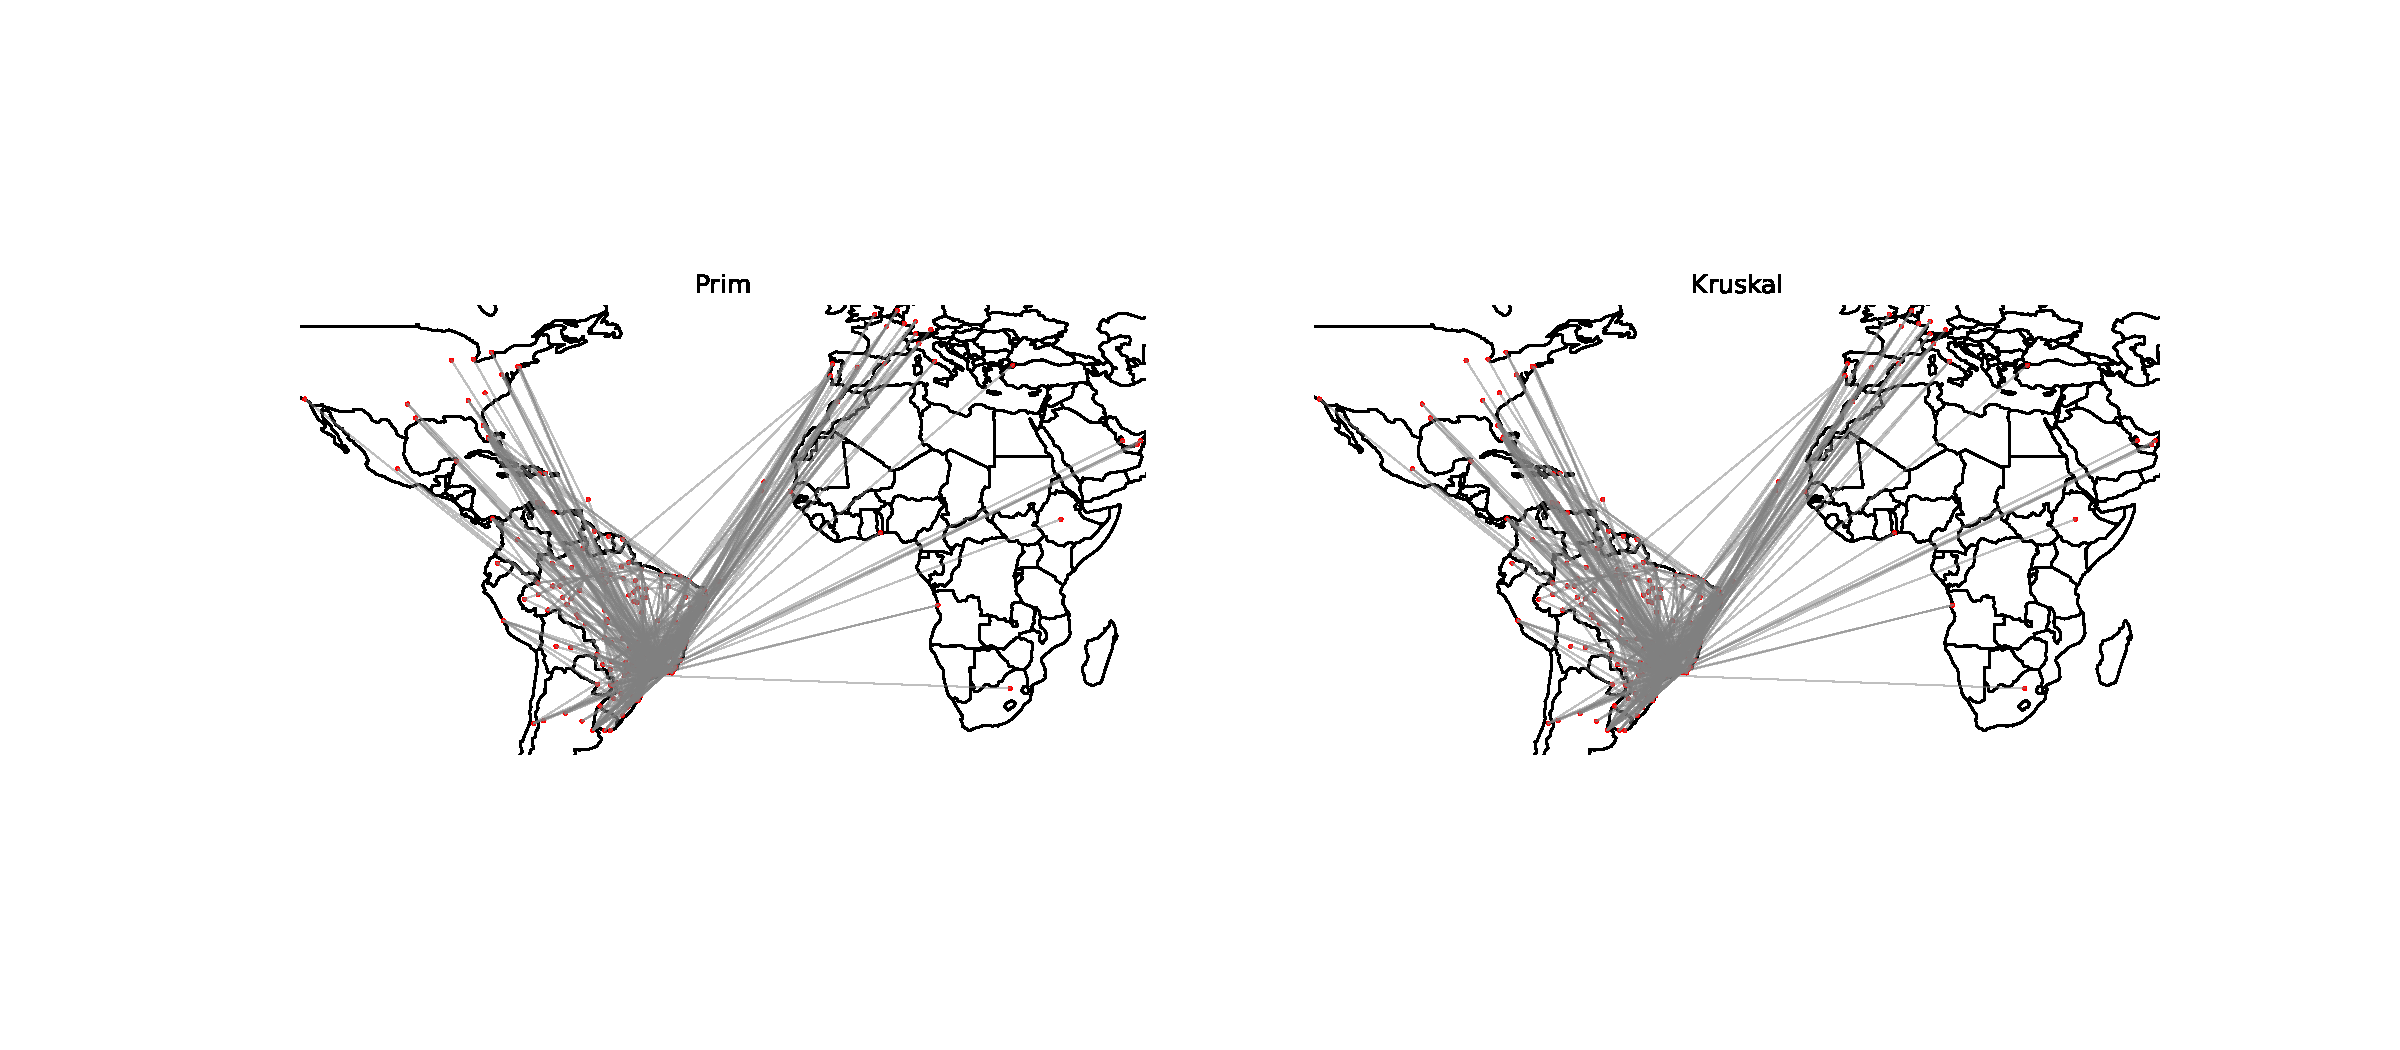
\includegraphics[width=\textwidth]{figs/world_time_mst_0.pdf}
    \end{figure}
\end{frame}

\begin{frame}{Prim x Kruskal - Duração do Voo}
    \begin{figure}[ht]
        \centering
        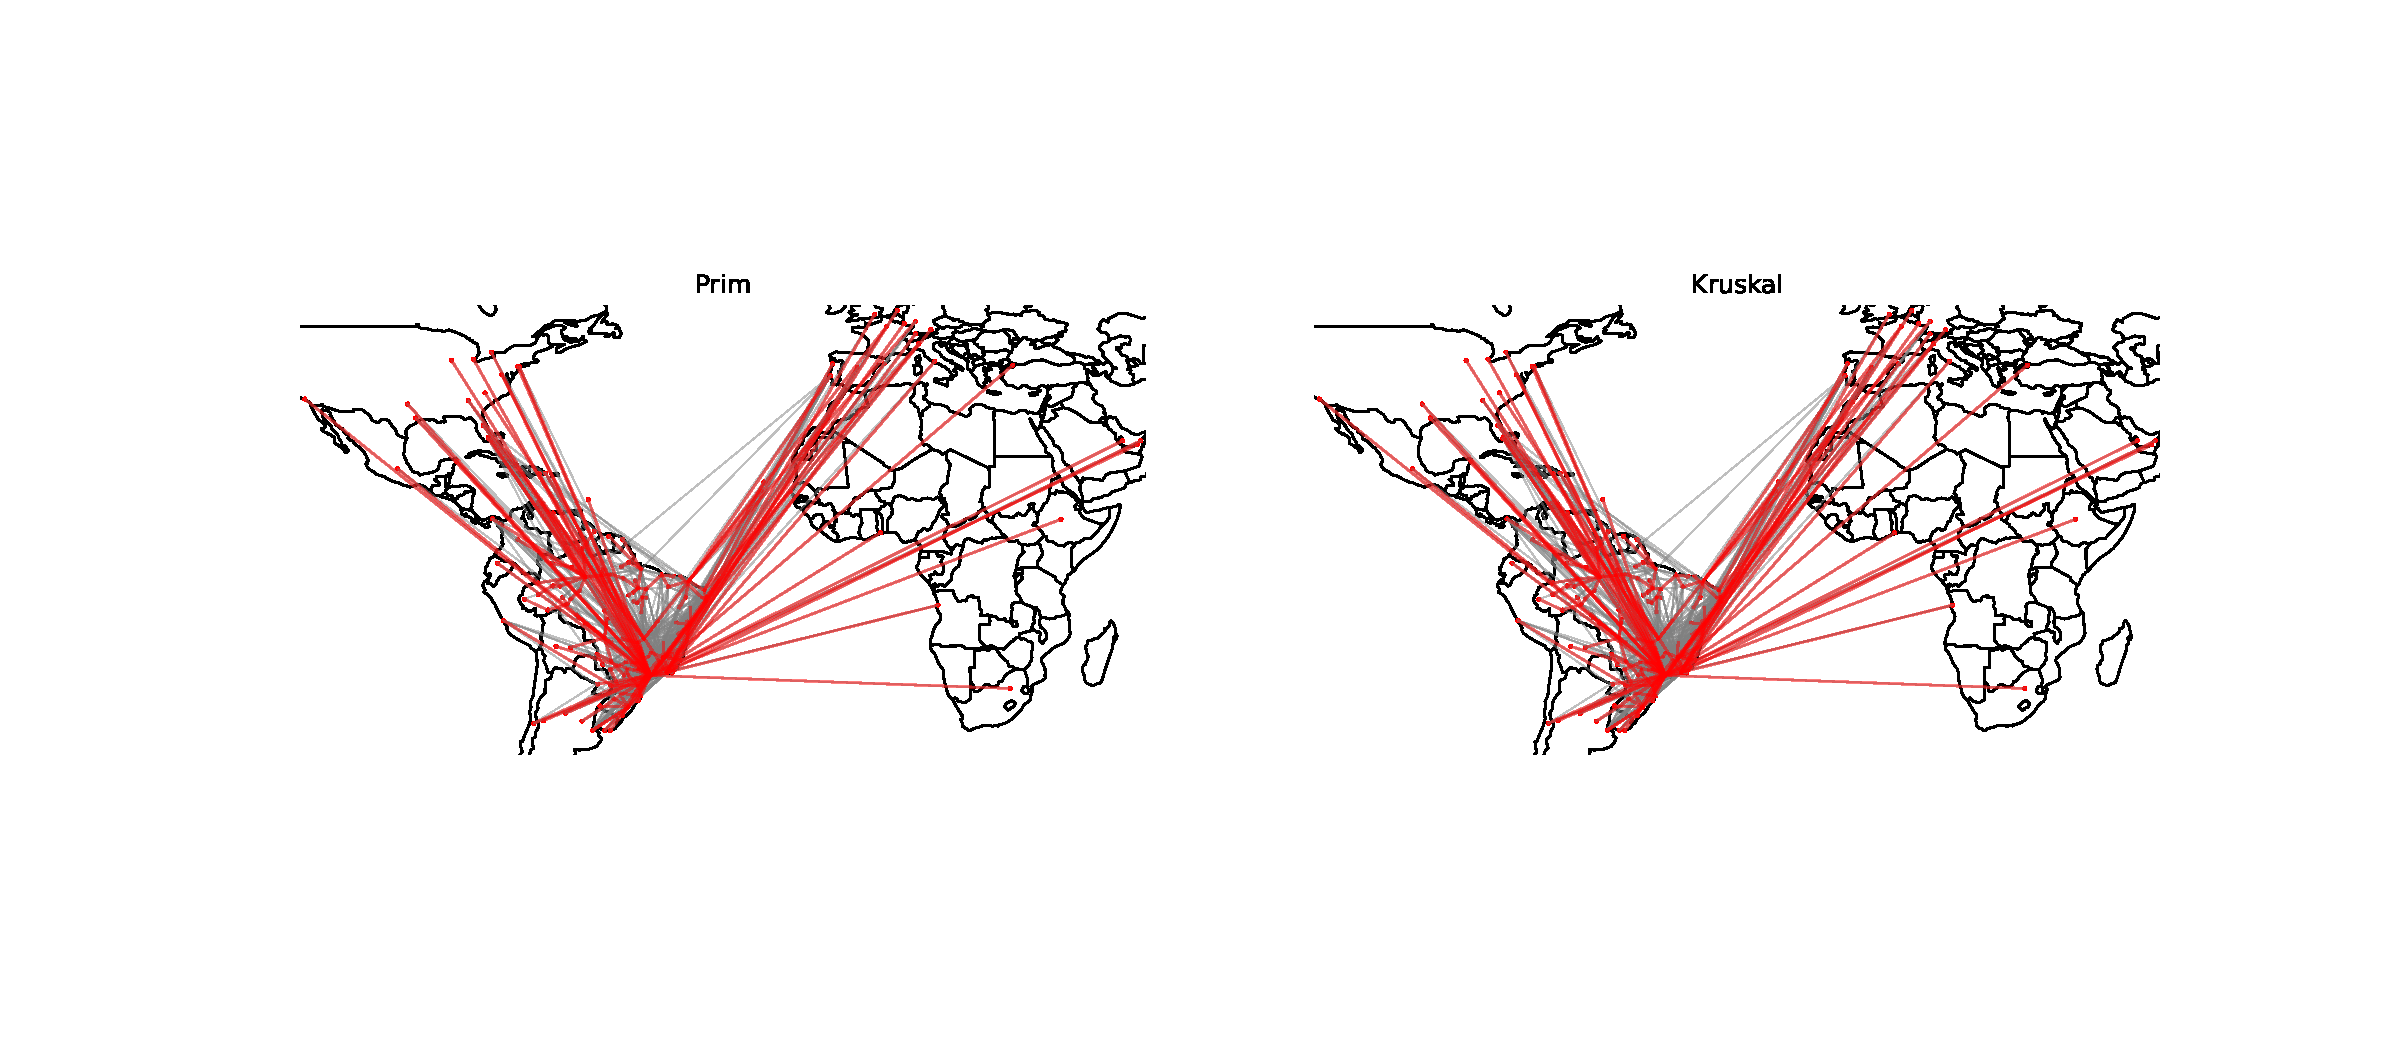
\includegraphics[width=\textwidth]{figs/world_time_mst_1.pdf}
    \end{figure}
\end{frame}

\begin{frame}{Prim x Kruskal - Duração do Voo - Brasil}
    \begin{figure}[ht]
        \centering
        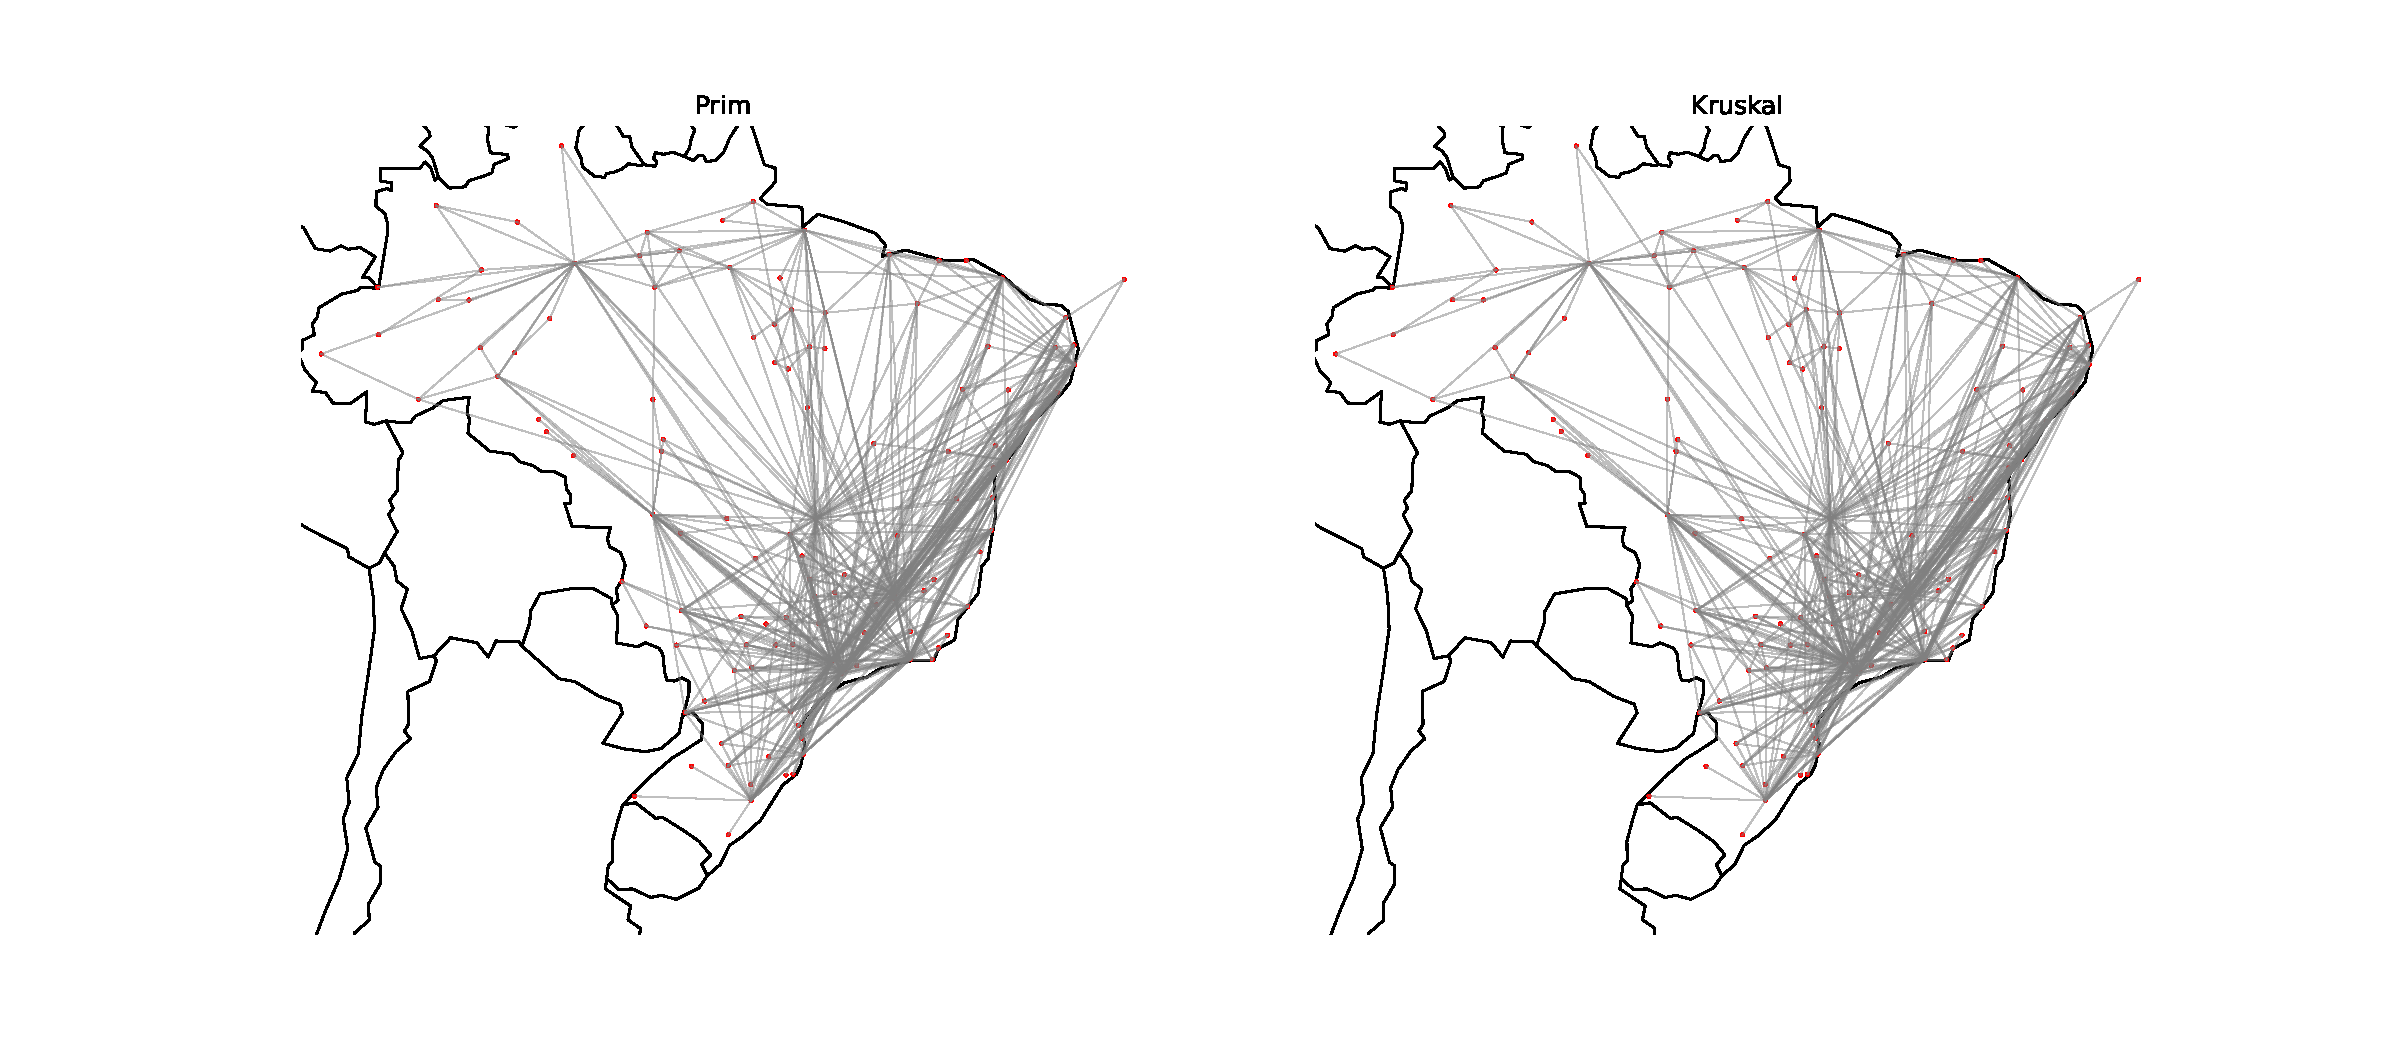
\includegraphics[width=\textwidth]{figs/brasil_time_mst_0.pdf}
    \end{figure}
\end{frame}

\begin{frame}{Prim x Kruskal - Duração do Voo - Brasil}
    \begin{figure}[ht]
        \centering
        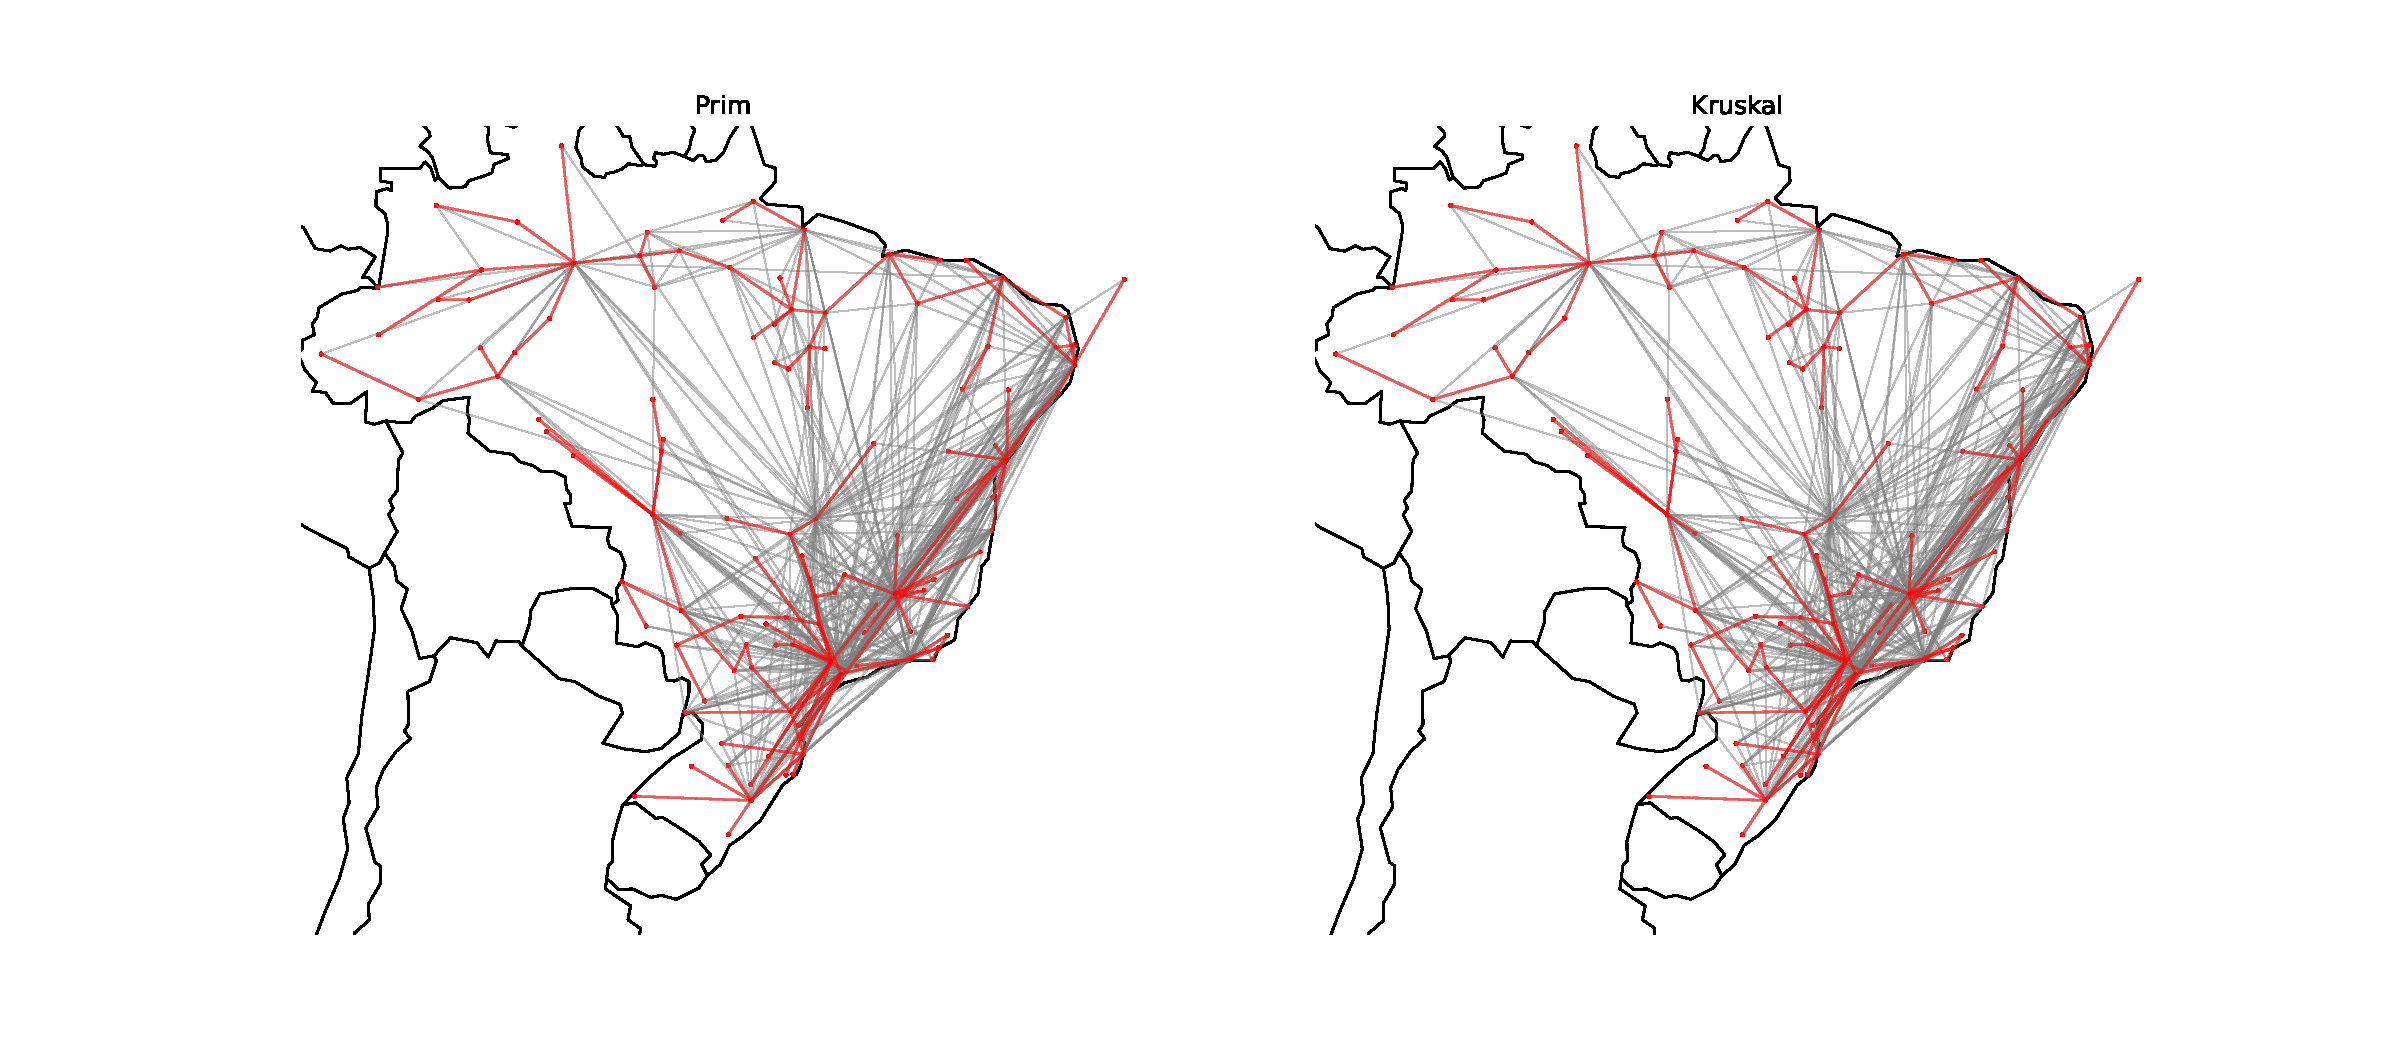
\includegraphics[width=\textwidth]{figs/brasil_time_mst_1.pdf}
    \end{figure}
\end{frame}

\begin{frame}{Duração x Distância - Brasil}
    \begin{figure}[ht]
        \centering
        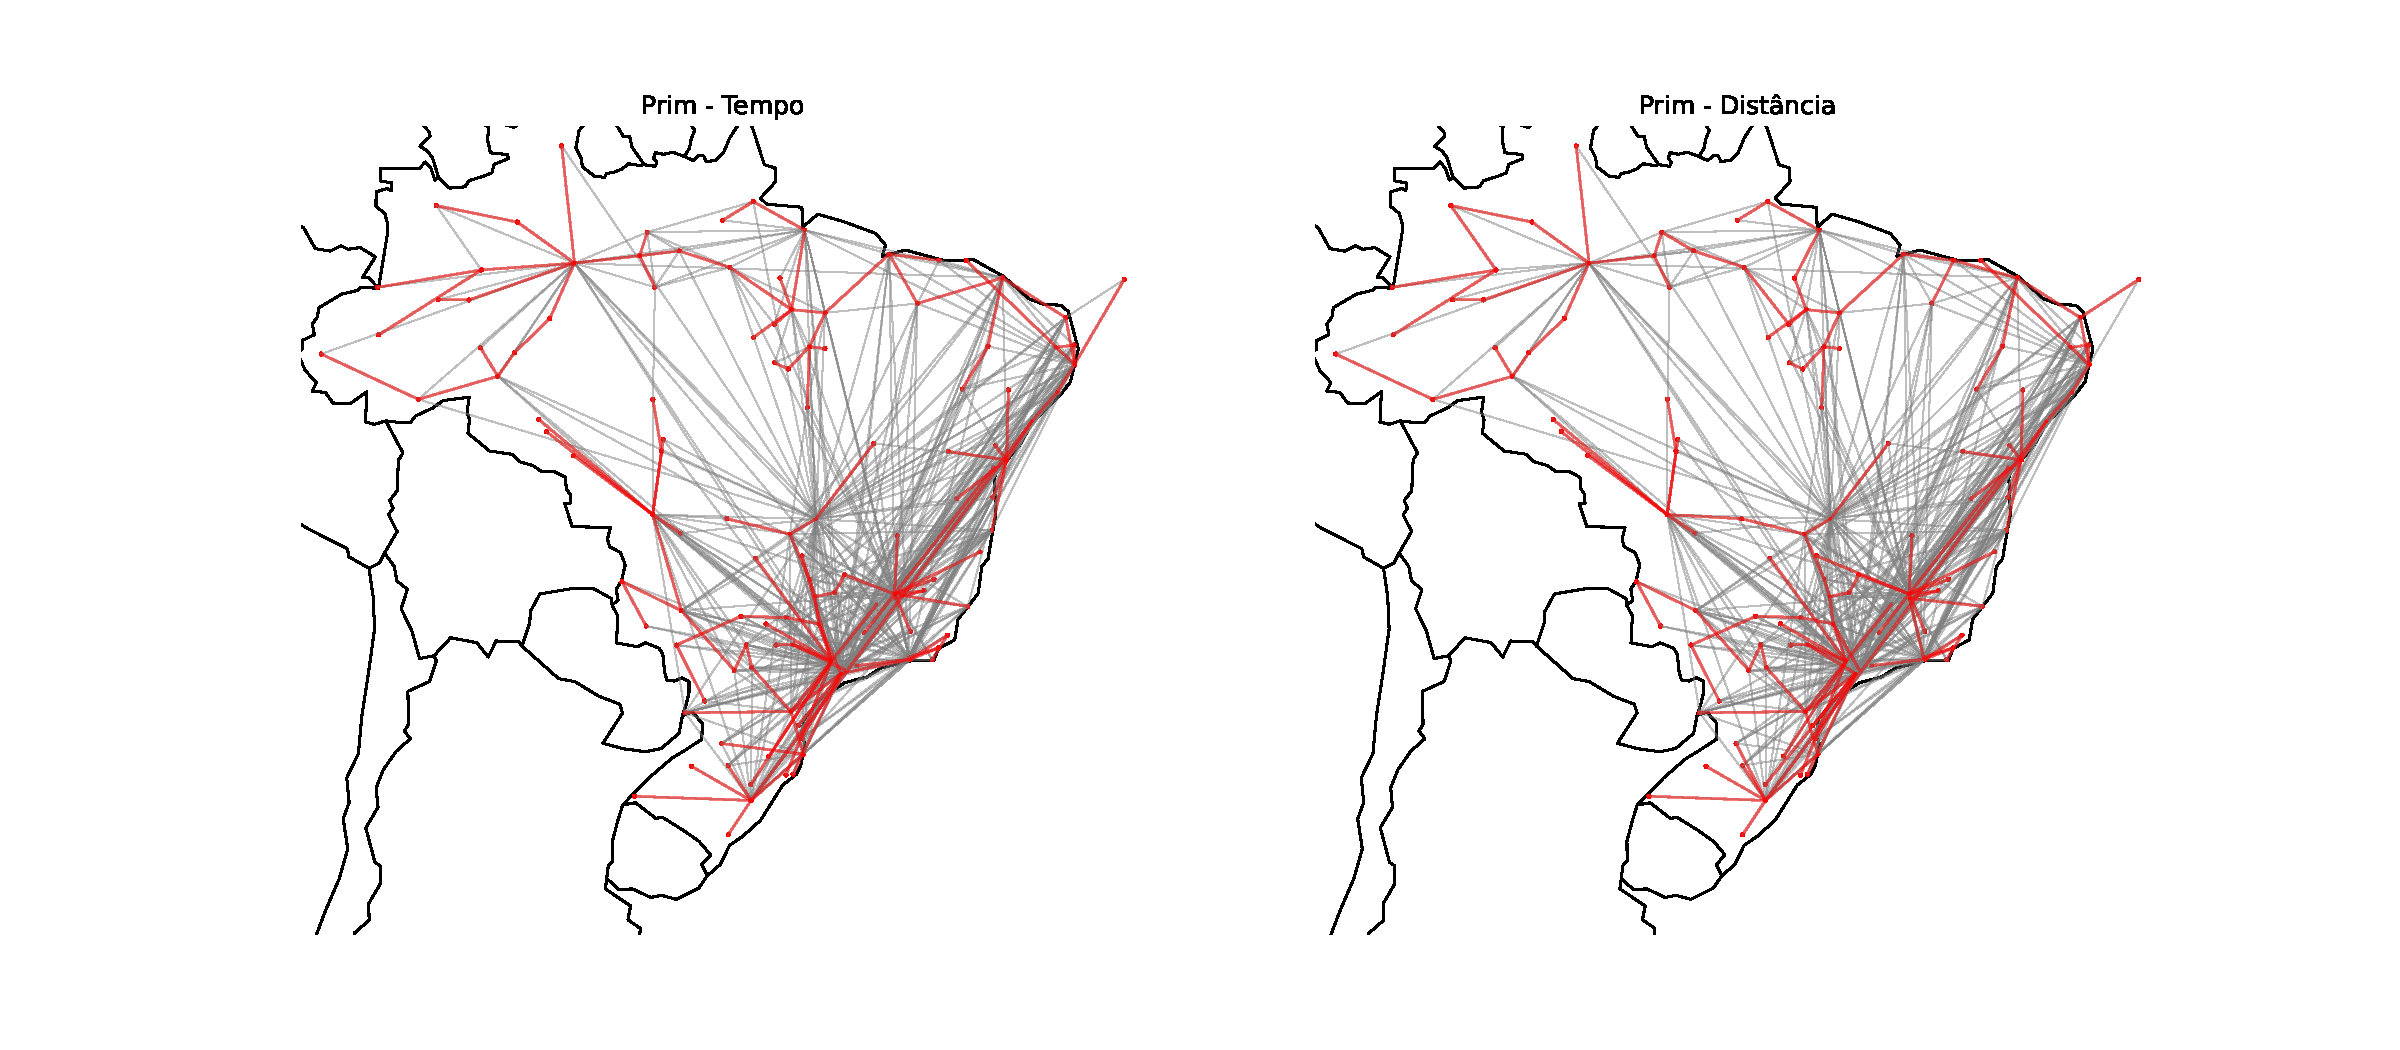
\includegraphics[width=\textwidth]{figs/brasil_time_x_distance_mst_1.pdf}
    \end{figure}
\end{frame}

\begin{frame}{Duração x Distância - Fernando de Noronha}
    \begin{figure}[ht]
        \centering
        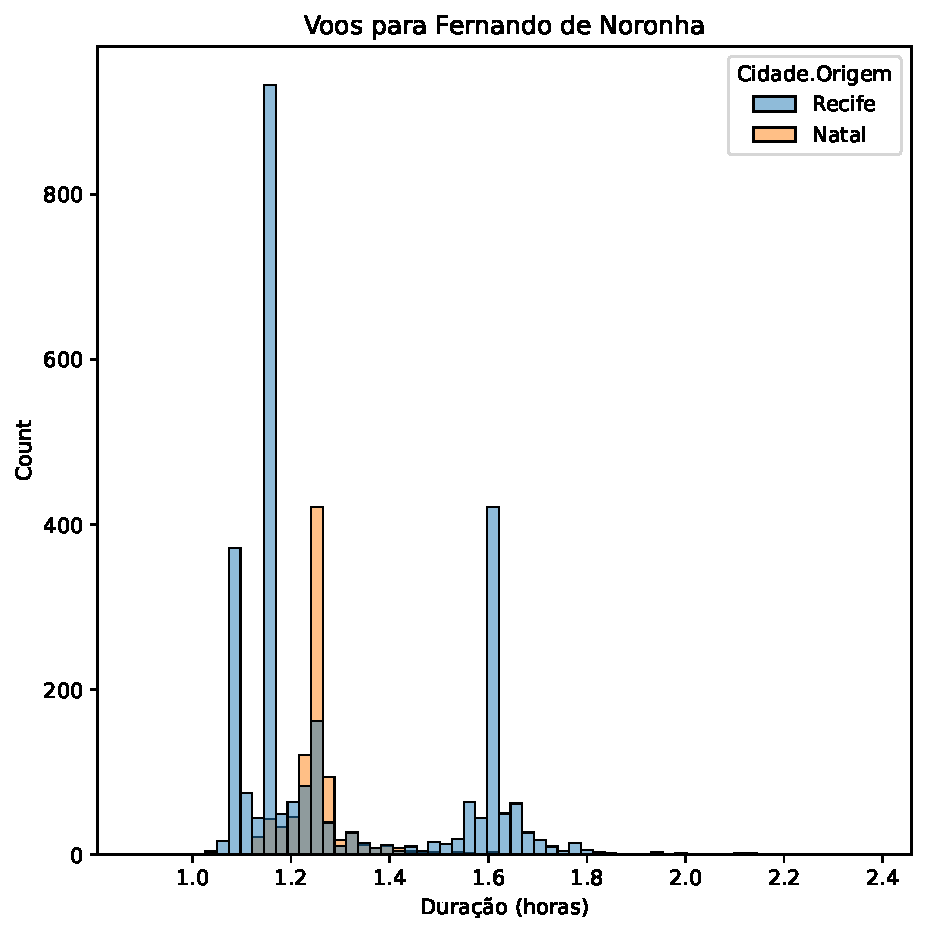
\includegraphics[width=0.5\textwidth]{figs/histograma_fernando_noronha.pdf}
    \end{figure}
\end{frame}


\end{document}
